\documentclass{beamer}
\usetheme{Hannover}


\usepackage{algorithm}
\usepackage{algorithmic}
\usepackage{amsmath}
\usepackage{amssymb}
\usepackage{amsthm}
\usepackage[ngerman,english]{babel}
\usepackage{centernot} 
\usepackage{color}
\usepackage{dsfont}
\usepackage{graphicx}
\usepackage[utf8]{inputenc}
\usepackage{import}
\usepackage{standalone}
\usepackage{qtree}

\usepackage{hyperref}

\title{Integral infeasibility and testing total dual integrality}
\author{David L.Applegate, William Cook S.Thomas McCormick}

\newcommand{\N}{\ensuremath{\mathds{N}}}
\newcommand{\R}{\ensuremath{\mathds{R}}}
\newcommand{\red}[1]{\textcolor{red}{#1}}

\setlength{\itemsep}{-2pt}


\begin{document}

%Presentation of the problem

\begin{frame}
	\frametitle{Linear system of Barahona and Mahjoub problem}
	\begin{itemize}
		\item
		Let $s$ be the following linear system for a graph $D$ :\\
		$\forall$ directed circuit $C$ of $D$, $\sum\{x_e:e\in C\}\geqslant 1$\\
		$x_e\geqslant 0$ for each arc $e$ of $D$ 
		\item
		Example : 
		\begin{figure}
			\centering
			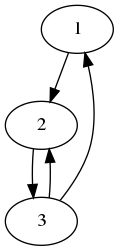
\includegraphics[width=1.5cm]{images/example1.png}
		\end{figure}
		The associated linear system may be written:\\
		$\begin{pmatrix} -1 & -1 & -1 & 0\\ 0 & -1 & 0 & -1 \end{pmatrix}_A \begin{pmatrix} x_{1->2}\\ x_{2->3}\\ x_{3->1}\\ x_{3->2} \end{pmatrix}_x \leqslant \begin{pmatrix} -1 & -1 \end{pmatrix}_b$\\
	\end{itemize}
\end{frame}
	
\begin{frame}
	\frametitle{Barahona and Mahjoub problem}
	Let $D_5$, the complete symetric directed graph on 5 nodes :
	\begin{figure}
		\centering
		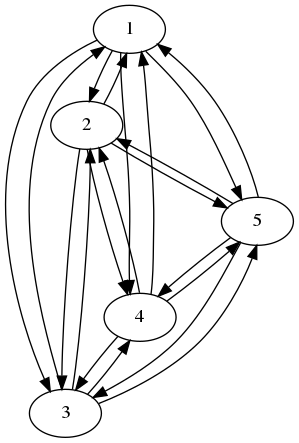
\includegraphics[width=3cm]{images/D5.png}
	\end{figure}
	Is $s$ for $D_5$ totally dual integral?
\end{frame}

%Feedback sets

\begin{frame}
	\frametitle{Feedback sets}
	\begin{itemize}
		\item A 0-1 solution is a solution such that : $\forall e\in D, x_e\in\{0,1\}$
		\item Such a solution corresponds to a subset of arcs $S\subseteq D$ which meets every circuit in $D$
		\item $S$ is called a \textit{feedback set}
		\item Example
		\begin{figure}
			\centering
			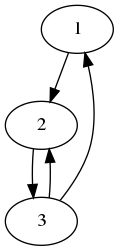
\includegraphics[width=1.5cm]{images/example1.png}
		\end{figure}
		In this example, $\{2->3\}$ is a feedback set.
	\end{itemize}
\end{frame}

\begin{frame}
	\frametitle{Lemma3}
	\begin{itemize}
		\item $D_5$ has 84 directed circuits, so we want to reduce that number before computing anything. For that we will need the lemma 3.
		\item Lemma 3 : Suppose that $D$ is a directed graph with arcs $ij$ and $ji$, that $D_1$ is $D$ with $ji$ deleted, and $D_2$ is $D$ with $ij$ deleted. If $s$ is totally dual integral for both $D_1$ and $D_2$, it is totally dual integral for $D$.
		\item
		Example :
		\begin{figure}
			\centering
			$D$ : 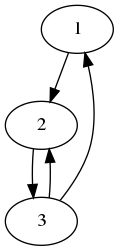
\includegraphics[width=1.5cm]{images/example1.png}
			$D_1$ : 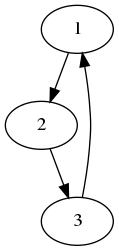
\includegraphics[width=1.5cm]{images/D1.png} 
			$D_2$ : 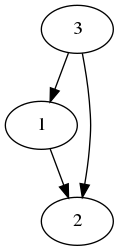
\includegraphics[width=1.5cm]{images/D2.png}
		\end{figure}
	\end{itemize}
\end{frame}

\begin{frame}
	\frametitle{From $D_5$ to $K_5$}
	\begin{itemize}
		\item Thanks to lemma 3, we can conclude that if for each orientation of $K_5$, $s$ is totally dual integral, then it is totally dual integral for $D_5$
		\item 
		\begin{figure}
			\centering
			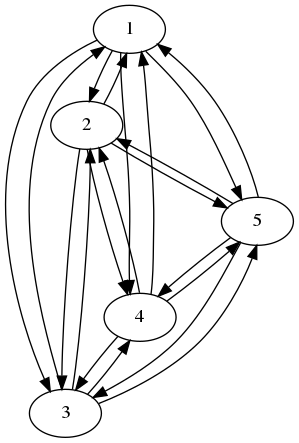
\includegraphics[width=2cm]{images/D5.png}
			->
			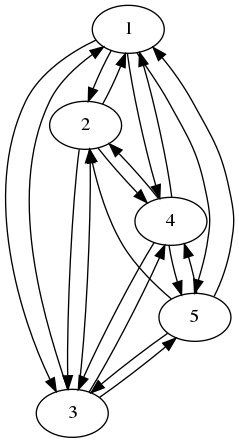
\includegraphics[width=1.5cm]{images/d5-1.png}
			->
			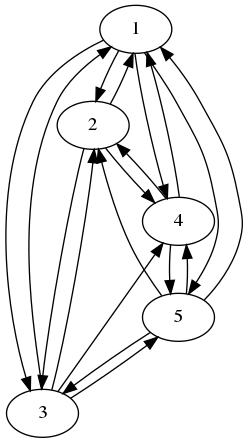
\includegraphics[width=1.5cm]{images/d5-2.png}
			...
			->
			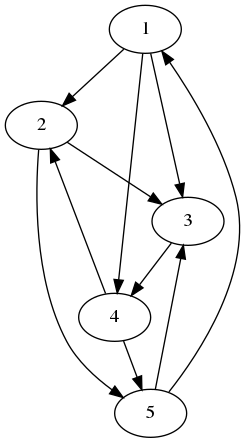
\includegraphics[width=1.5cm]{images/d9.png}
		\end{figure}
		\item This reduces the maximum number of circuits for each orientation to 12.
	\end{itemize}
\end{frame}

\begin{frame}
	\frametitle{Barahona and Mahjoub lemma}
	\begin{itemize}
		\item We now want to reduce the number of orientation to fully treat. For that we need the lemma 4, from Barahona and Mahjoub.
		\item Lemma 4 : Let $D$ be an orientation of $K_5$. Then if either some node of D meets all directed circuit or some arc is in no directed circuit, $s$ is totally dual integral for $D$.
		\item By checking for lemma 4 and isomorphism, there only remain 3 distinct orientation of $K_5$ to treat.
	\end{itemize}
\end{frame}

\begin{frame}
	\frametitle{The final computation}
	\begin{figure}
		\centering
		$D(12)$: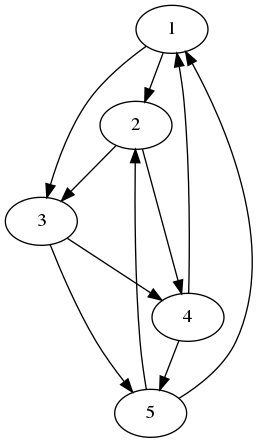
\includegraphics[width=2cm]{images/d12.png}
		$D(10)$: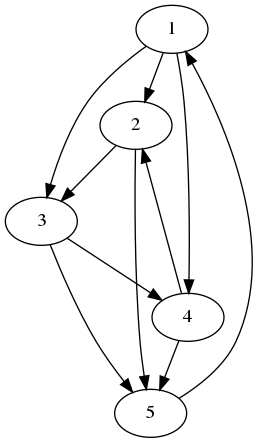
\includegraphics[width=2cm]{images/d10.png}
		$D(9)$: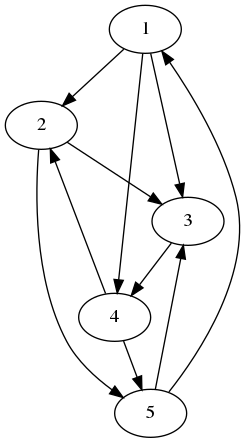
\includegraphics[width=2cm]{images/d9.png}
	\end{figure}
	Compute times for each run :
	\begin{itemize}
		\item $D(12)$ : 14h 33mn 21s
		\item $D(10)$ : 2h 52mn 7s
		\item $D(9)$ : 1h 6mn 3s
	\end{itemize}
\end{frame}
%%%%%%%%%%%%%%%%%%
%%%%%%    %%%%%%%%
%%%%%%%%%%%%%%%%%%

\end{document}
